\chapter{Financial Reports}\label{ch:financial_reports}

Only a few financial statements are needed to get a good overall picture of a school's or district's finances. These are:
\begin{itemize}[nosep]\OnehalfSpacing\medskip%
  \item The enacted Annual Budget and Interim Reports
  \item The audited Comprehensive Annual Financial Report (CAFR)
  \item The Local Control Accountability Plan (LCAP)
\end{itemize}\noindent%

This appendix uses financial statements from the Los Altos School District (LASD) to illustrate what a public or a charter school's financial statements look like.

\section{Annual Budgets}\label{sec:annual-budgets}
Budgets, in California, are the first of four important financial documents that schools produce during a fiscal year. For any given fiscal year, which runs from July 1 to June 30, the first financial document produced is the annual budget, a forward looking financial statement, which is approved before the end of the prior fiscal year.\footnote{Since a school's budget needs to be approved before the state budget is finalized, it is guaranteed that a school's budget will need to be modified after it has been approved.} Next are two (unaudited) interim reports, one in December, and another in March,  which track how well the school or district is adhering to the approved annual budget, and finally, after a certified public accountant has audited the school or district, a comprehensive annual financial report (CAFR). State law requires that an independent auditor certify this retrospective account of the school or district's financial activity as being an accurate representation of the school's finances for the previous fiscal year.

A more detailed examination of one district's finances are provided in \prettyref{ch:ca-school-financing}.  A very detailed and thorough exposition of public school financing is in \textcite{Aguinaldo.etal2021} which is updated annually (except for the pandemic year of 2021).

% Figure~\vref{fig:LASD_All_Funds_Summary}, \titleref{fig:LASD_All_Funds_Summary}, is a very high-level summary of a school's or a district's budget. It's a snapshot of what the district's revenues are expected to be, roughly where that revenue is expected to come from, what the district's expenses are expected to be, and whether revenue and expenses are expected to be in balance. It is the rough equivalent of a business income statement.\footnote{Schools group their finances by funds. Most of their revenue goes into the general fund, and most of their expenses come out of the general fund. Some transactions must by law be accounted for in different funds. The three largest are the General Fund, the Special Revenue Fund, and the Capital Projects Fund, and together they account for virtually all of the financial activity of LASD.\@ Other schools may have a different set of funds, but all contain a General Fund that is the primary fund for their day-to-day financial activities.}

% \begin{figure}
%   \centering
%   \caption{\textit{LASD 2019–20 All Funds Summary}}\label{fig:LASD_All_Funds_Summary}
%   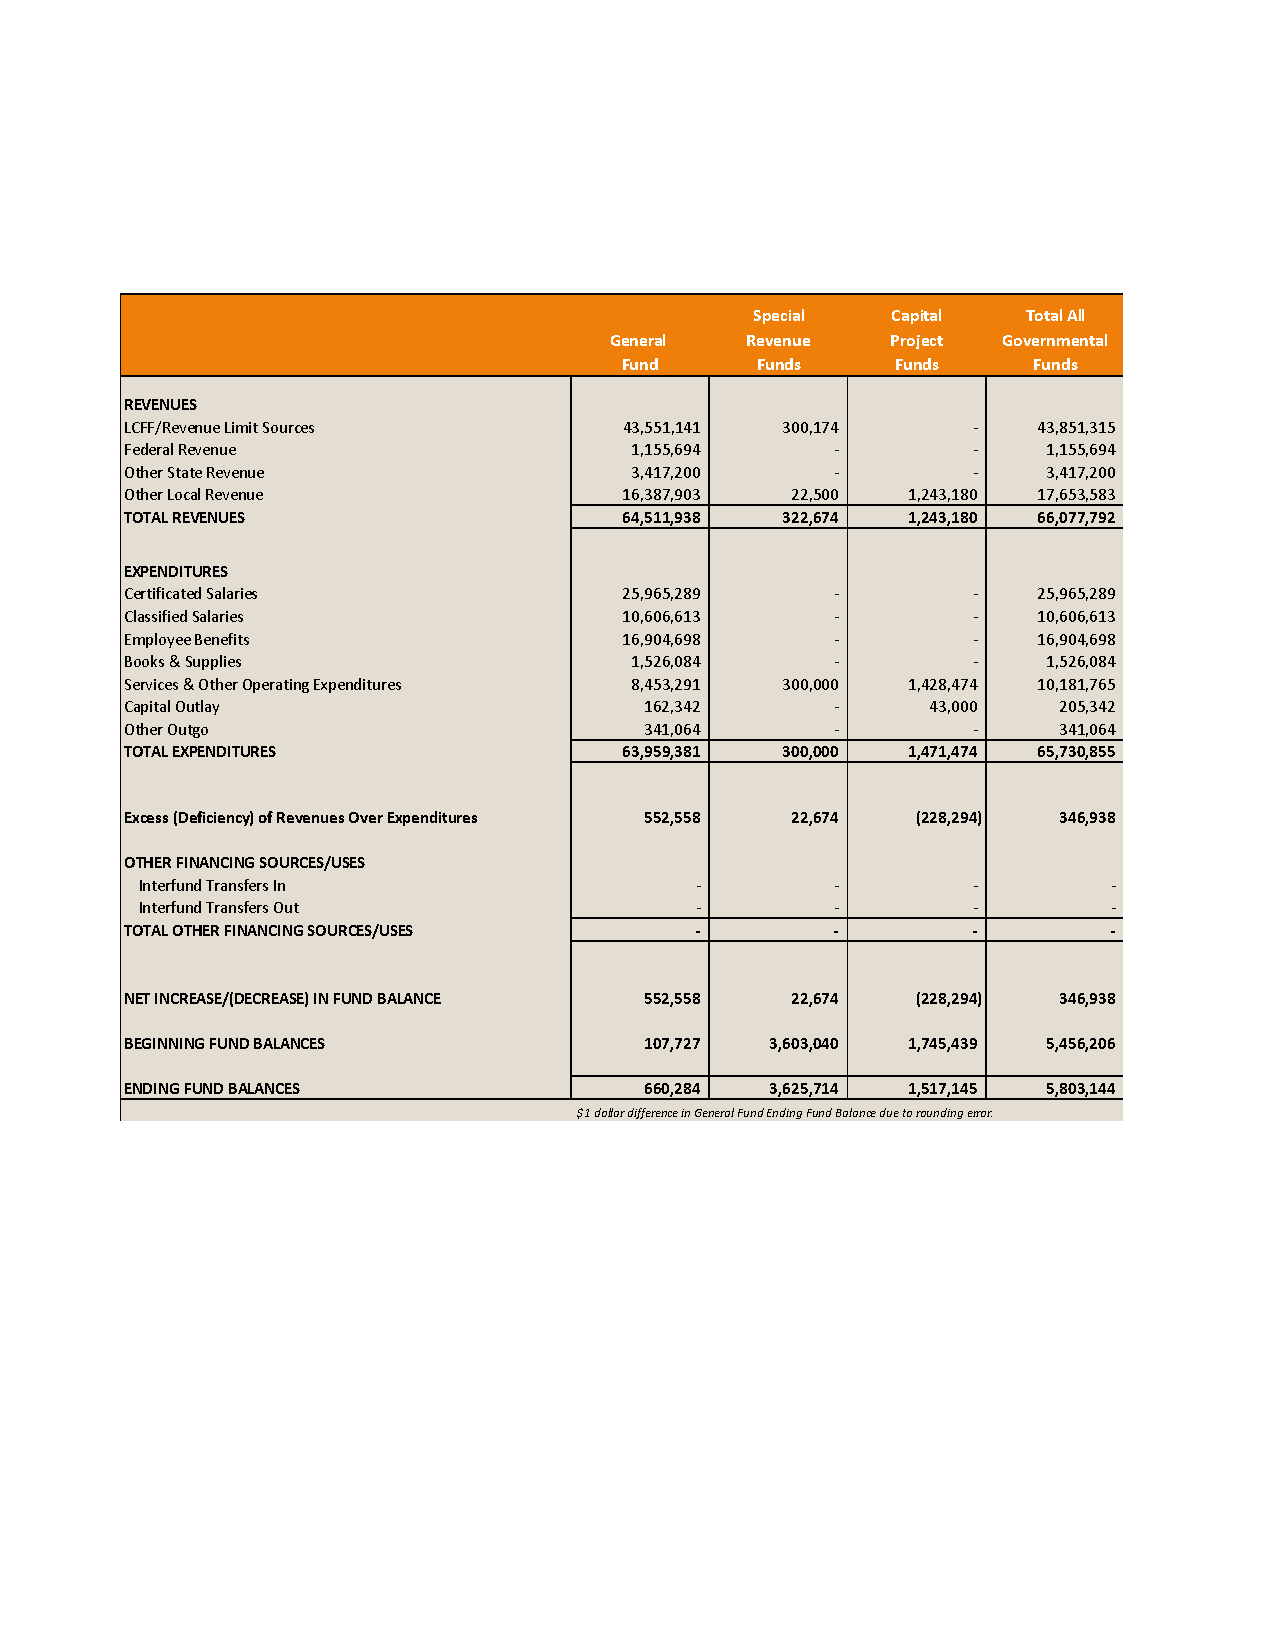
\includegraphics[width=433pt]{LASD_2019-20_All_Funds_Summary}\\ %chktex 8
%   \footnotesize\raggedright\textcite[38]{Kenyon2019}.
% \end{figure}

% Because Figure~\vref{fig:LASD_All_Funds_Summary},~\titleref{fig:LASD_All_Funds_Summary}, is a snapshot, detecting unusual changes year-to-year is not possible. Changes are detectable using  Figure~\vref{fig:net-position} which compares fiscal two years. However, with just a budget summary, one can nonetheless note some interesting ratios, for example, the percentage of expenses spent on salaries and benefits. For LASD in 2021–20, this is 80.18\% which is in line with what is typical of elementary school districts in California. One can calculate the state-wide average for all districts for 2019–20 using the Data Table at \url{www.ed-data.org/state/CA}, and that comes out to 83.71\%. So, LASD spends a little less on salaries and benefits than the average elementary school district in California does.

% Calculating this ratio brings up a general issue: What is an appropriate comparison group? In this particular case, the Ed-Data web site does not have county-level financial data, so the only comparison which can easily be made is at the state level. But should the state-level comparison group be all districts, or just elementary school districts? Should ``basic aid'' districts, also called ``community-funded'' districts, districts whose property tax revenues exceed their LCFF entitlement, be included or not? Again, the Data Table tab on \url{www.ed-data.or/state/CA} does not filter by type of district (although the Graph tab does), so, in this case, using just the Ed-Data data, our choices are forced since we cannot use state-level data.

% The other common financial business report is the balance sheet, which identifies assets and liabilities. In the educational world, this is the statement of net position. Figure~\vref{fig:net-position} shows LASD's assets and liabilities at the end of the 2019–20 school year. Note that unlike a balance sheet, a statement of net position for schools (and other governmental entities) does not balance; assets are not exactly equal to liabilities.\footnote{Business accountants achieve this seemingly low probability equality by adding a fudge factor, \textit{owner's equity}, so that \texttt{\textit{assets = liabilities + equity}} always, exactly.}

% As an example of a number which stands out and is therefore worth investigating, is the large increase in Capital Assets, year over year, an increase of \$132M (line 3 of~\vref{fig:net-position},~\titleref{fig:net-position}). In \citetitle{Kenyon2021}, six notes appear immediately after Figure~\ref{fig:net-position}, and these provide an explanation for the increase: LASD purchased a property whose cost was \$134.9M net of \$2.7M in depreciation. This purchase shows up again in line 1 of Figure~\vref{fig:Capital_Assets} and explains the enormous 9052\% increase in the value of LASD's largest asset in FY2019, land.

% In addition, the \citetitle{Kenyon2021} contains a section, on pp. 19–45, called \textit{Notes to the Basic Financial Statements}. Theses notes are an integral part of the certified, audited annual statement, just as they are in audited financial reports in the business world; they cannot be omitted, and must be accurate and complete.  Note 7B of \textcite[7]{Kenyon2021}, General Obligation (GO) Bond Anticipation Notes (BANs), explains how LASD uses a common
% technique to convert general obligation bonds into cash: issue BANs, backed by general obligation bonds, and payable when those GO bonds are issued.\footnote{One reason this makes sense is that interest rate on BANs is less than the interest rate of GO bonds, so LASD makes money by issuing BANs to pay off GO bonds. In a different situation, school districts issue tax revenue anticipation notes (TRANs) because property taxes are paid by taxpayers semi-annually and salaries are paid monthly, so districts often and predictably do not have the cash on hand to pay their employees. The solution is to issue TRANs backed by anticipated revenue, and are paid off when the school or district receives the funds.}

% It's important to remember is that although changes in finances can be complicated, they should also be adequately explained in a transparent and complete CAFR. When the documents are incomplete or opaque is when serious concerns should be raised. % chktex 13

% Within a CAFR are five summaries of financial tables that go one level deeper than the All Funds Summary. These are
% \begin{itemize}[nosep]\OnehalfSpacing\medskip%
%     \item Summary of Net Position (Figure~\vref{fig:net-position})
%     \item Change in Net Position  (Figure~\vref{fig:Change_Position})
%     \item Net Costs of Services   (Figure~\vref{fig:Cost_Services})
%     \item Capital Assets          (Figure~\vref{fig:Capital_Assets})
%     \item Long-term Liabilities   (Figure~\vref{fig:Long-term_Liabilities})
%   \end{itemize}\medskip%

% \begin{figure}
%   \centering
%   \caption{\textit{LASD YE 2020 Summary of Net Position}}\label{fig:net-position}
%   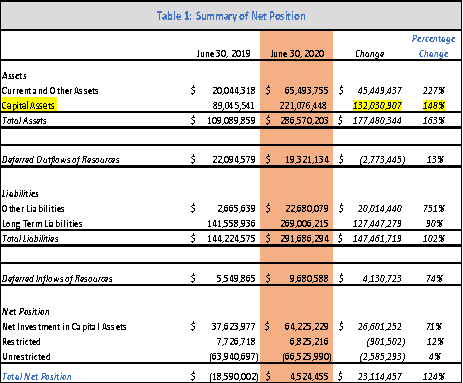
\includegraphics[width=433pt]{CAFR-YE2020_Summary_of_Net_Position}\\
%   \footnotesize\raggedright\\textcite[6]{Kenyon2021}.
% \end{figure}

% \begin{figure}
%   \centering
%   \caption{\textit{LASD YE 2020 Change of Net Position}}\label{fig:Change_Position}
%   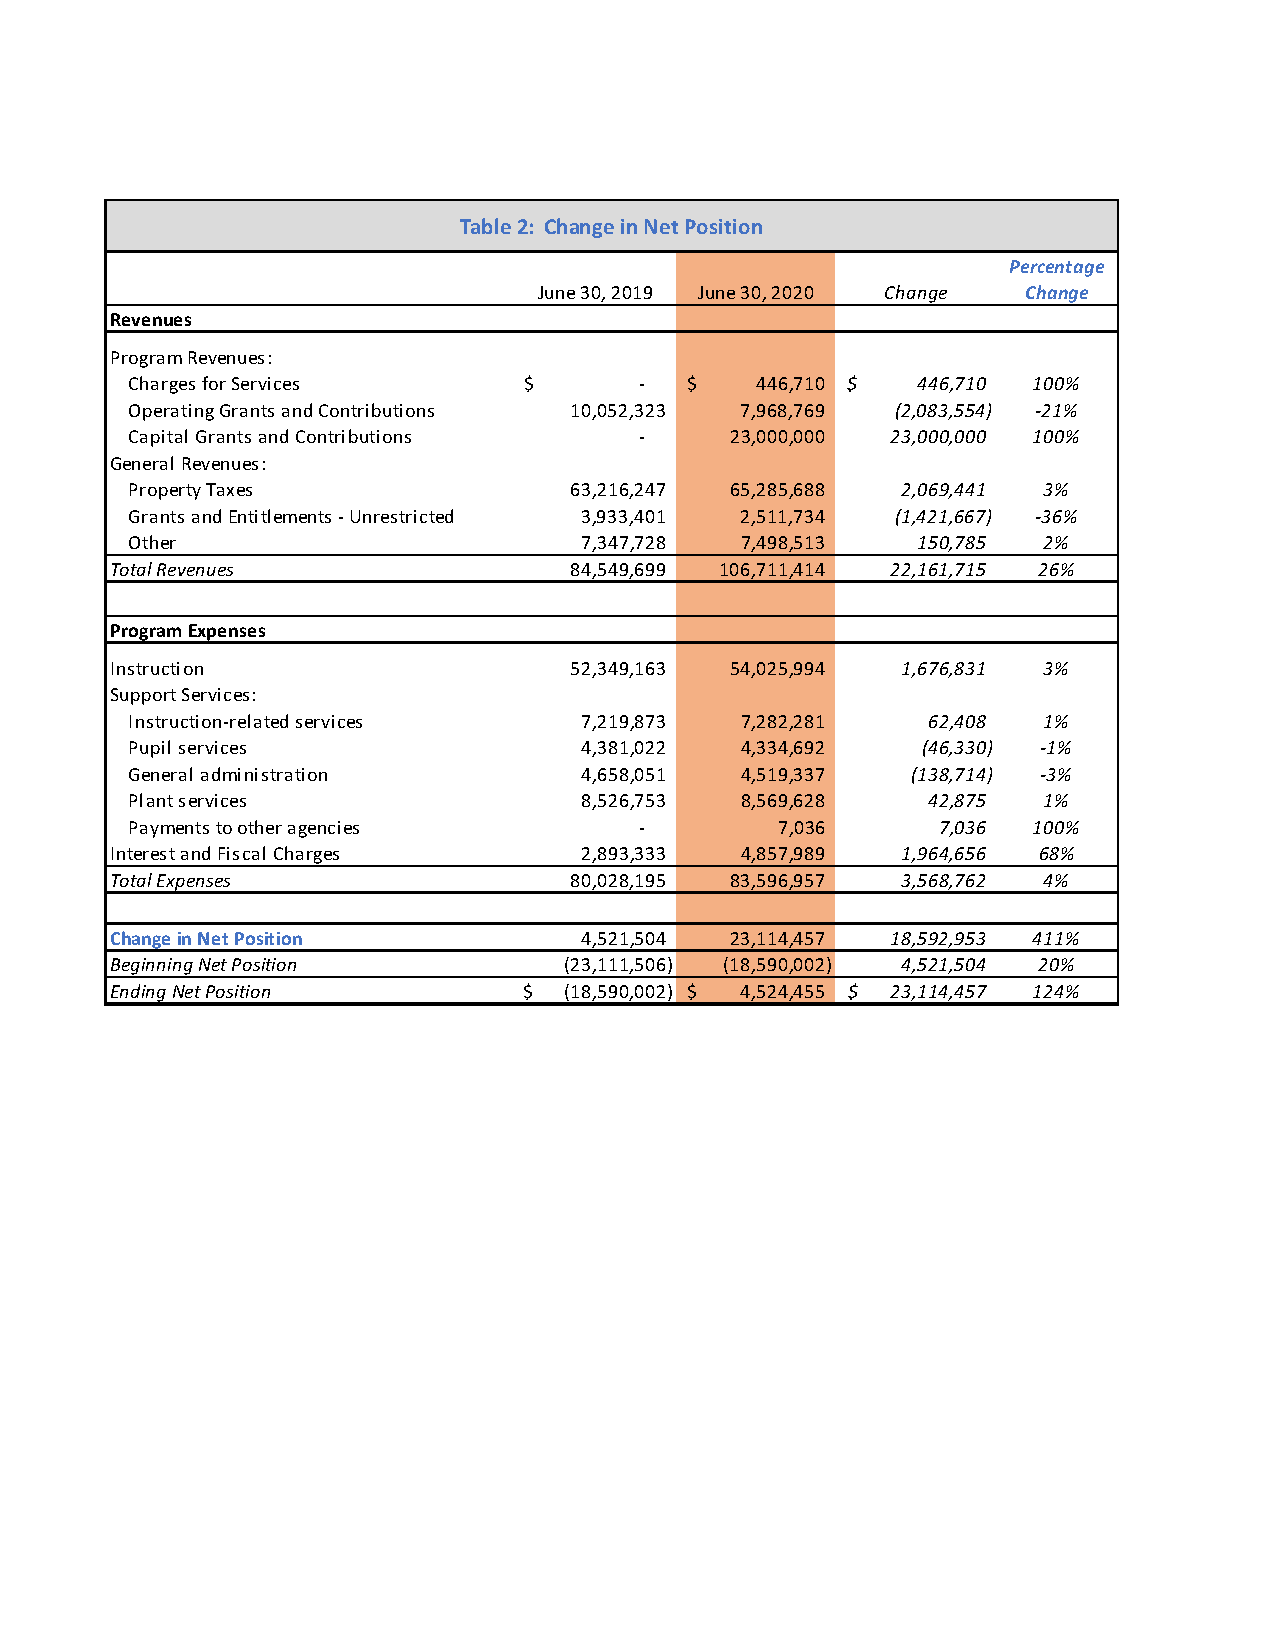
\includegraphics[width=433pt]{CAFR-YE2020_Change_in_Net_Position}\\
%   \footnotesize\raggedright\textit{Note:} \textcite[7]{Kenyon2021}.
% \end{figure}

% \begin{figure}
%   \centering
%   \caption{\textit{LASD YE 2020 Net Cost of Services}}\label{fig:Cost_Services}
%   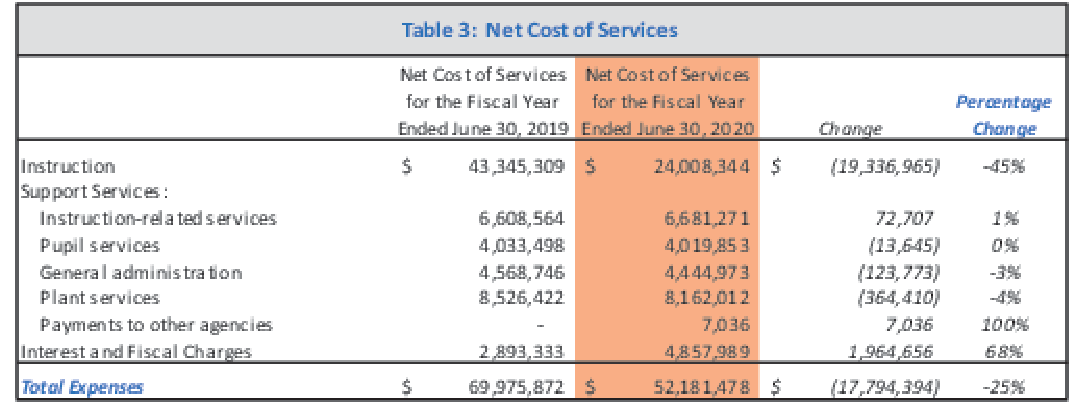
\includegraphics[width=433pt]{CAFR-YE2020_Net_Cost_of_Services}\\
%   \footnotesize\raggedright\textcite[9]{Kenyon2021}.
% \end{figure}

% \begin{figure}
%   \centering
%   \caption{\textit{LASD YE 2020 Capital Assets}}\label{fig:Capital_Assets}
%   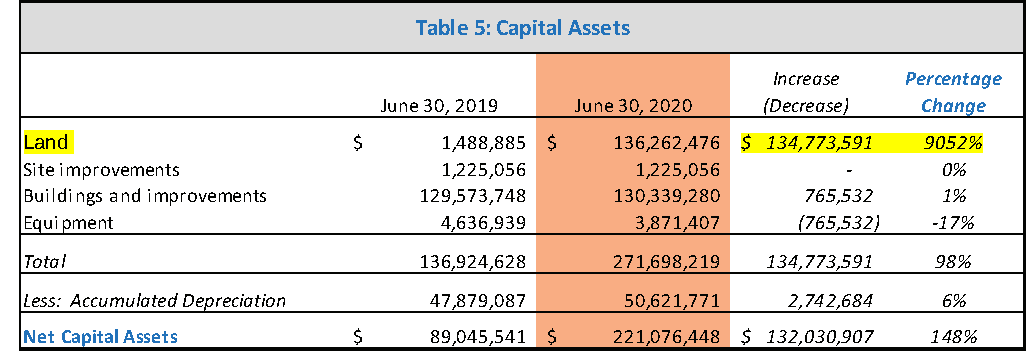
\includegraphics[width=433pt]{CAFR-YE2020_Capital_Assets}\\
%   \footnotesize\raggedright\textcite[10]{Kenyon2021}.
% \end{figure}

% \begin{figure}
%   \centering
%   \caption{\textit{LASD YE 2020 Long-term Liabilities}}\label{fig:Long-term_Liabilities}
%   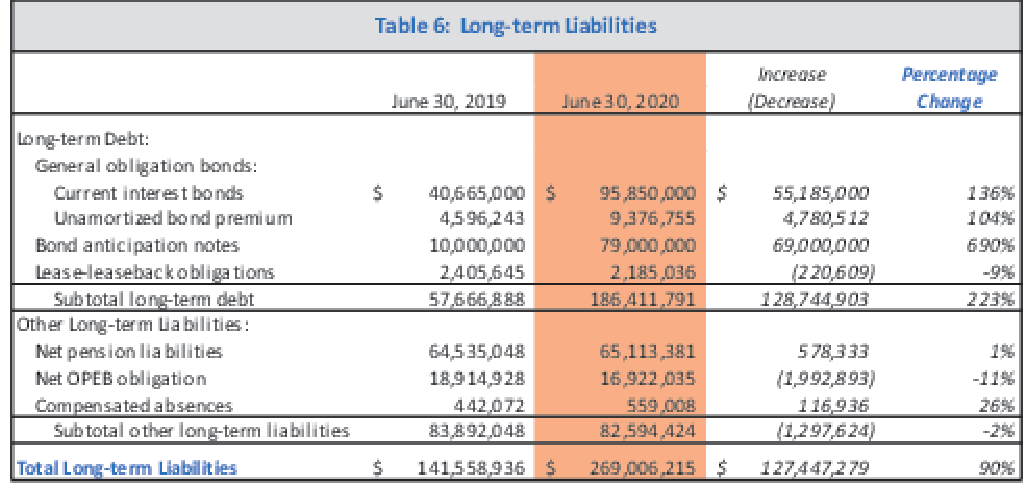
\includegraphics[width=433pt]{CAFR-YE2020_Long-term_Liabilities}\\
%   \footnotesize\raggedright\textcite[11]{Kenyon2021}.
% \end{figure}%

% LASD rolls up its detailed financial data into a single multi-year summary, as shown in Figure~\vref{fig:multi-year-proj}. In addition to purely financial data, the multi-year summary includes the key
% assumptions that were behind the numbers. In fact, the first section of Figure~\ref{fig:multi-year-proj} is only assumptions, and it is those assumptions which drive the numbers in sections 2–4. The value of this summary is that it captures in one table the key data needed to make budgetary decisions and thus might serve as a template for what data is important. 

% \begin{figure}[!t]
%   \centering
%   \caption{\textit{LASD 2019–20 Multi-Year Projection}}\label{fig:multi-year-proj}
%   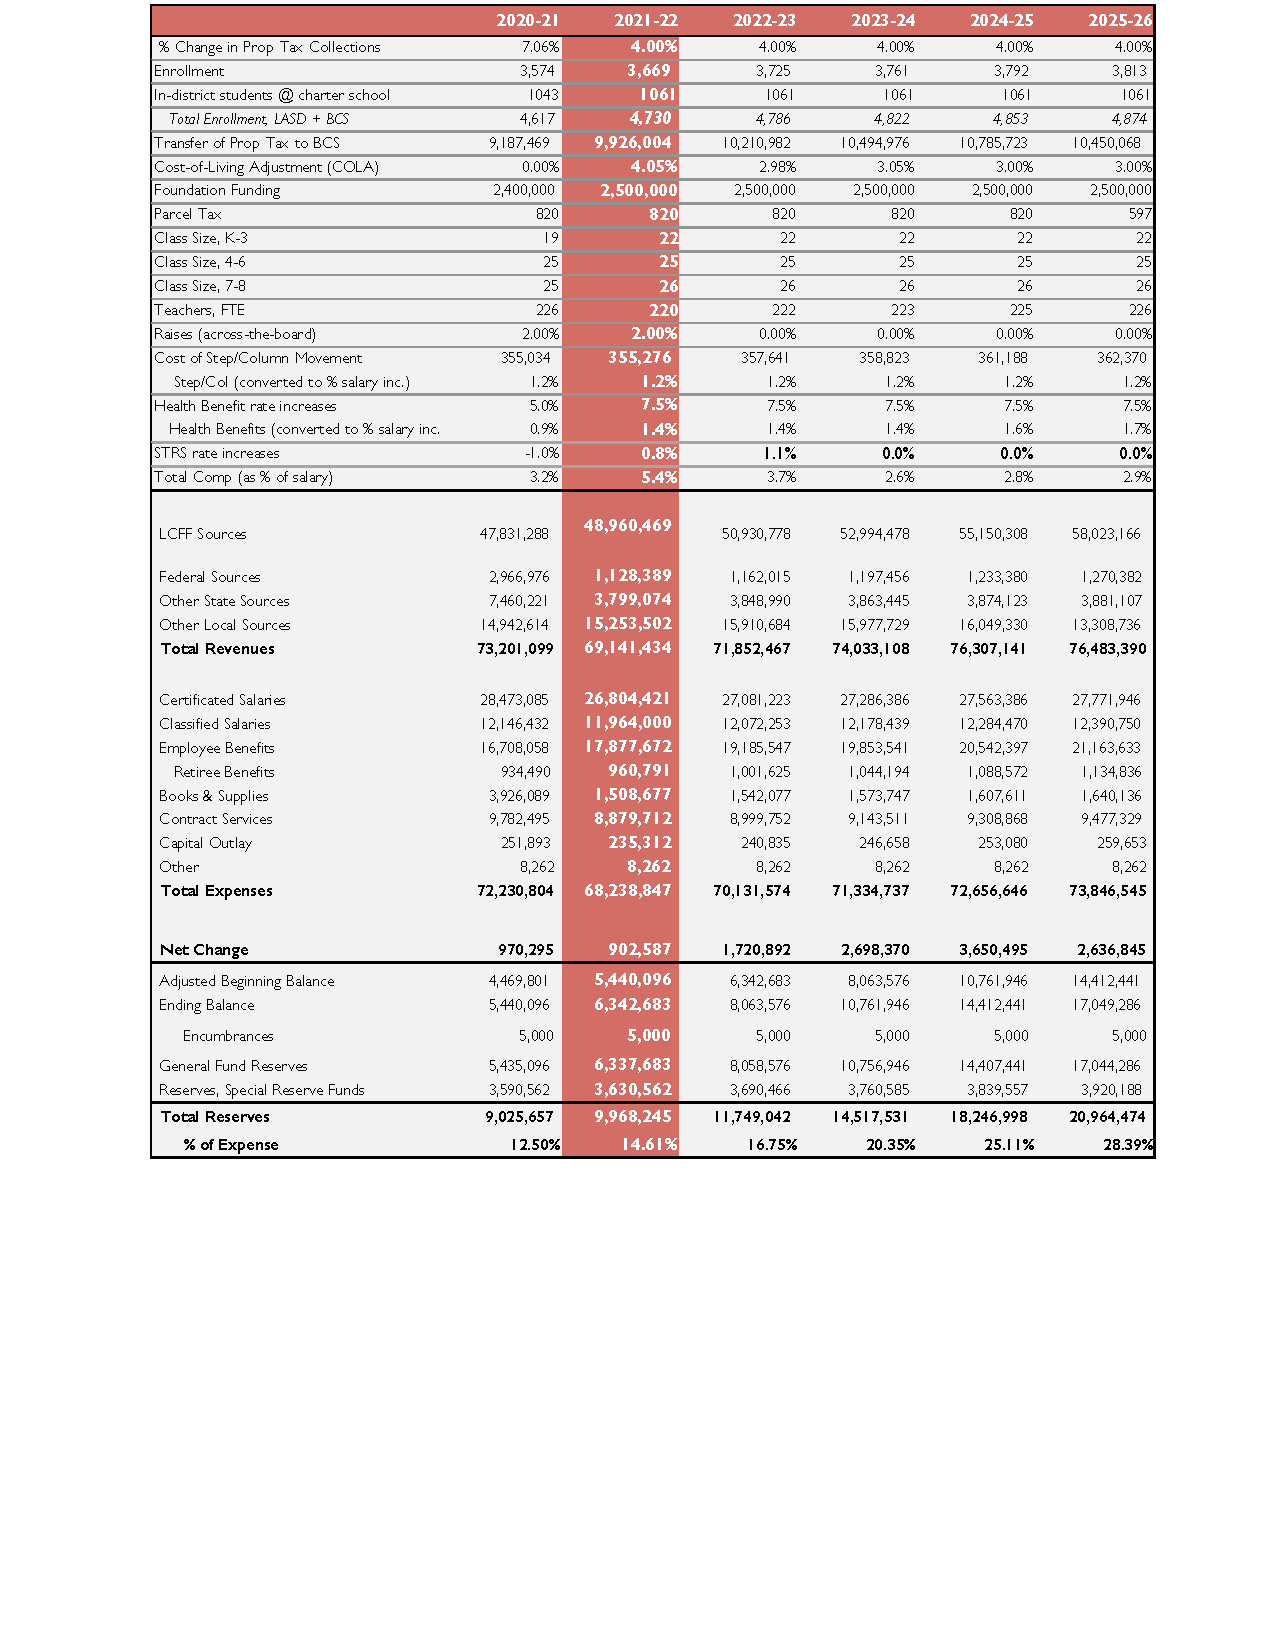
\includegraphics[width=433pt]{LASD_Multi_Year_Projection}\
%   \footnotesize\raggedright\\textcite[137]{Kenyon2021a}
% \end{figure}\bigskip%

%%% Local Variables:
%%% mode: latex
%%% TeX-master: "Rocketship_Education-An_Exploratory_Public_Policy_Case_Study"
%%% End:
